\section{Arquitectura capa de aplicación}
{Esta capa, es la capa de arquitectura del proyecto orientada al aplicación, aquí se plasma la estructura de la aplicación del software soportado en componentes reusables e interfaces de comunicación \cite{archimate}.}

	\subsection{Punto de vista de comportamiento de aplicación}
	{ El comportamiento de aplicación muestra cómo se componen internamente una aplicación, es útil para diseñar el comportamiento principal del sistema o componentes, e identificar la superposición funcional de estas \cite{archimate}.\\
	\newpage
		
		\textbf{Modelo}\\
		\begin{figure}[H]
			\centering
			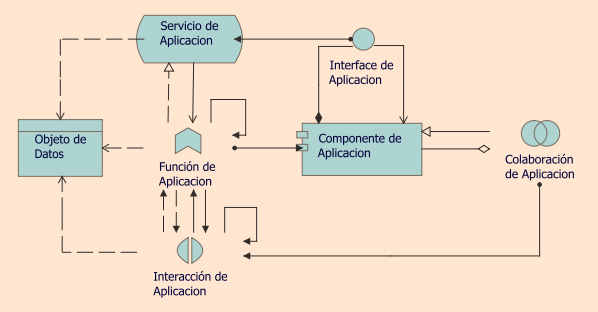
\includegraphics[width=0.8\linewidth]{development/comportamientoapp.png}
			\caption{Metamodelo Comportamiento de Aplicación}
		\end{figure}
		\begin{center}
			\textbf{Fuente:} Colosoft E.U: Documento CasoColoSoft.
		\end{center}
		\hfill \break
			
		\textbf{Caso:} Los componentes de aplicación son:
		
		\begin{itemize}
			\item Gestionar préstamo
			\item Realizar préstamo
			\item Registrar usuarios
		\end{itemize}
		
		\begin{figure}[H]
			\centering
			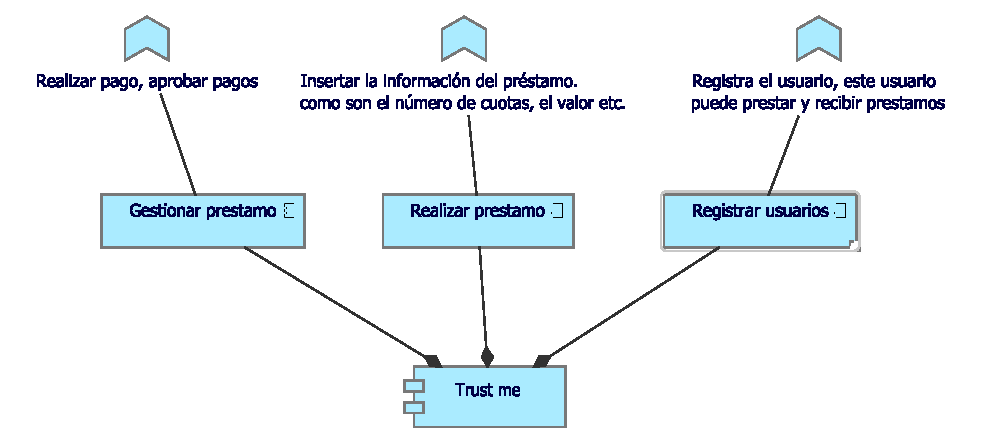
\includegraphics[width=0.6\linewidth]{development/comportamientoapp.pdf}
			\caption{Comportamiento de Aplicación}
		\end{figure}
		\begin{center}
			\textbf{Fuente:} Propia.
		\end{center}
	}
	
	\subsection{Punto de vista de cooperación de aplicación}
	{La  cooperación de aplicación describe las relaciones entre los componentes en términos de flujo de información o en términos de los servicios que estos proveen o usan. Este punto de vista también es usado para expresar la cooperación interna u orquestación de servicios que juntos soportan la ejecución de un proceso de negocio \cite{archimate}.\\
		
		\textbf{Modelo}\\
		\begin{figure}[H]
			\centering
			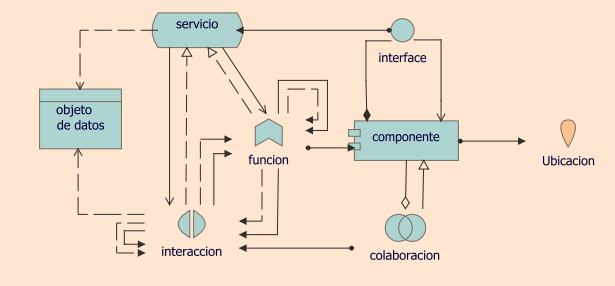
\includegraphics[width=0.8\linewidth]{development/cooperacionapp.png}
			\caption{Metamodelo Cooperación de Aplicación}
		\end{figure}
		\begin{center}
			\textbf{Fuente:} Colosoft E.U: Documento CasoColoSoft.
		\end{center}
		\hfill \break
		
		\textbf{Caso:} Se presenta  el modelo de la aplicación, y los componentes visibles para los usuarios, que le permitirán interactuar con la misma, siendo estos, la gestión de los préstamos, la realización de los préstamos y el registro de usuarios.\\
		
		\begin{figure}[H]
			\centering
			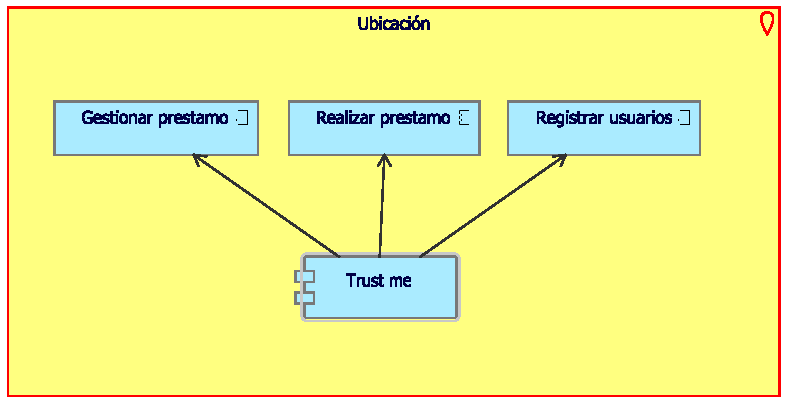
\includegraphics[width=0.7\linewidth]{development/cooperacionapp.pdf}
			\caption{Cooperación de Aplicación}
		\end{figure}
		\begin{center}
			\textbf{Fuente:} Propia.
		\end{center}
	}
	
	\subsection{Punto de vista de uso de aplicación}
	{Es utilizada para el diseño de la aplicación donde se identificaran los servicios que serán requeridos y estarán disponibles, por el proceso de negocio y otras aplicaciones \cite{archimate}.\\
		
		\textbf{Modelo}\\
		\begin{figure}[H]
			\centering
			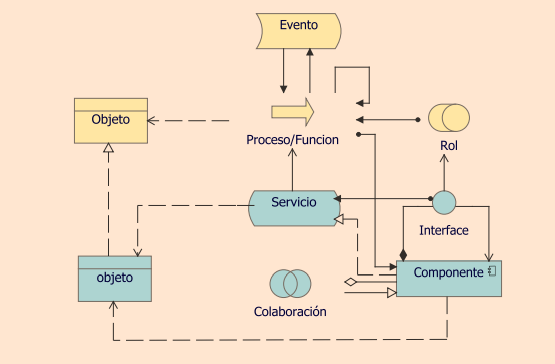
\includegraphics[width=0.7\linewidth]{development/usoapp.png}
			\caption{Metamodelo de Uso Aplicación}
		\end{figure}
		\begin{center}
			\textbf{Fuente:} Colosoft E.U: Documento CasoColoSoft.
		\end{center}
		
		\textbf{Caso:} Se presentan los principales servicios de la aplicación como lo son prestar y gestionar prestamos, los cuales son usados por los usuarios en el proceso del negocio.\\
		
		\begin{figure}[H]
			\centering
			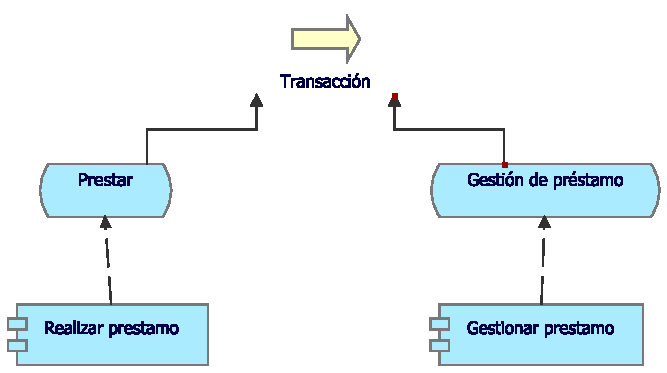
\includegraphics[width=0.8\linewidth]{development/usoapp.pdf}
			\caption{Uso Aplicación}
		\end{figure}
		\begin{center}
			\textbf{Fuente:} Propia.
		\end{center}
	}
	
